\chapter{Desarrollo del Proyecto}

\minitoc

\section{Introducción}

El presente capítulo detalla el proceso de desarrollo del proyecto realizado dentro de este Trabajo Fin de Grado. Tal como se ha comentado, el objetivo del proyecto era
proporciona al producto LUCA una herramienta gráfica para poder crear \emph{procesos}, es decir, poder encadenar consultas entre sí en base a sus valores de entrada y de salida.

\begin{figure}[H]
	\centering
	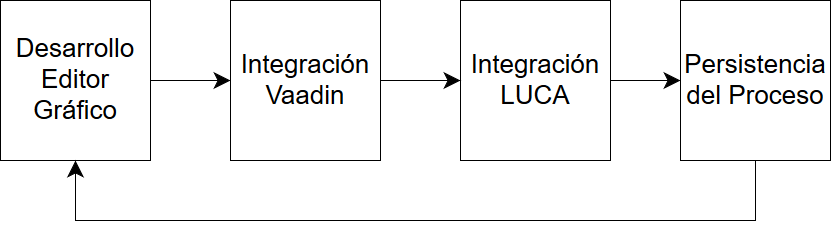
\includegraphics[width=\linewidth]{flujoDesarrollo.png}
	\caption{Flujo de Desarrollo}
	\label{fig:flujoDesarrollo}
\end{figure}

Para alcanzar este objetivo, se siguió el esquema de trabajo que se muestra en la Figura~\ref{fig:flujoDesarrollo}.

\begin{figure}[H]
	\centering
	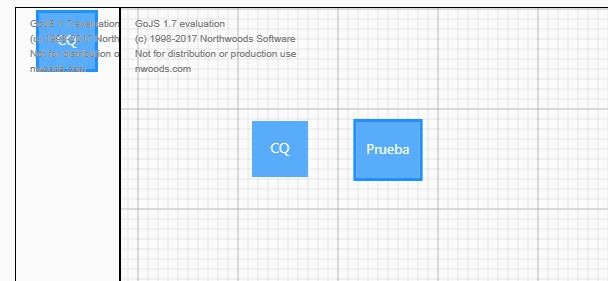
\includegraphics[width=\linewidth]{initalSampleEditor.jpeg}
	\caption{Primer Contacto Editor}
	\label{fig:initialSampleEditor}
\end{figure}

La primera etapa consistió en realizar un primer contacto con la herramienta \emph{GoJS}, para ello, se realizó una prueba de concepto donde se creaba un diagrama sencillo con cajas o nodos que se conectan entre sí (Figura~\ref{fig:initialSampleEditor}).

Con la prueba de concepto funcionando, la segunda etapa consistió en integrar el diagrama en \emph{GoJS} con el framework de \emph{Vaadin}. De esta forma se obtenía un editor gráfico de procesos implementado en \emph{Java}, que podía ser utilizado en cualquier proyecto \emph{Vaadin}.

La tercera etapa se centró en integrar dicho proyecto genérico \emph{Vaadin} en el producto LUCA.  El objetivo era ser capaz de mostrar el editor y poder interactuar con él y recibir los eventos ocurridos, de acuerdo con el patrón \emph{Modelo-Vista-Presentador} y la arquitectura de \emph{Vaadin}.

Por último, la cuarta etapa consistió en añadir la capa de negocio y de persistencia al modelo de datos de LUCA, creado específicamente para persistir \emph{procesos} y toda su jerarquía de clases.

Una vez acabadas las cuatro etapas de desarrollo, comenzó un curso de iteraciones para refinar el proyecto e ir dando la complejidad final al mismo, de forma que se fue completando toda la lógica de negocio, así como, el aspecto gráfico final.

Paralelamente a estas etapas, y en cuanto fue posible, se trabajó en la parte de ejecución de los procesos especificados desde el editor gráfico y almacenados en LUCA. Las siguientes secciones proporcionan detalles sobre la ejecución de cada etapa.

\section{Desarrollo del Editor Gráfico}

%% Describir los pasos, a nivel general, para crear el editor gráfico sencillo.
El editor gráfico utiliza \emph{GoJS} para crear toda la interfaz visual. Este framework (como ya se explicó en el apartado de documentación) utiliza \emph{templates} para definir el aspecto estético de los diferentes componentes. Por lo tanto, el primer paso, tras tener claro cómo debía de ser un primer boceto de interfaz, fue crear todos los \emph{templates} de los que se iba a componer.

El segundo paso, una vez conseguida la estética y estructura de elementos deseada, fue comprobar la funcionalidad del mismo, desde asegurar que al interactuar con el editor se creaban los eventos oportunos, hasta comprobar que los elementos se mostraban en pantalla tal y como se quería.

\begin{figure}[H]
	\centering
	\begin{lstlisting}[language=Java]
	myDiagram.nodeTemplate = $(go.Node, "Table", {
		locationObjectName : "BODY",
		locationSpot : go.Spot.Center,
		selectionObjectName : "BODY"
	}, new go.Binding("location", "loc", go.Point.parse)
	.makeTwoWay(go.Point.stringify),
	
		$(go.Panel, "Auto", {
			row : 1,
			column : 1,
			name : "BODY",
			stretch : go.GraphObject.Fill
		},
			$(go.Shape, "Rectangle", {
				fill : "#58ACFA",
				stroke : null,
				strokeWidth : 0,
				name : "rectangle",
				minSize : new go.Size(56, 56)
			}),
				$(go.TextBlock, "CQ Default", {
					margin : 10,
					textAlign : "center",
					font : "14px  Segoe UI,sans-serif",
					stroke : "white",
					editable : true
				}, new go.Binding("text", "name").makeTwoWay()
			)
		)
	);\end{lstlisting}
	\caption{\emph{Template} Prueba Editor Inicial}
	\label{fig:initialSampleEditorCode}
\end{figure}

La Figura~\ref{fig:initialSampleEditor} y la Figura~\ref{fig:initialSampleEditorCode} muestran el primer boceto de editor. La primera se corresponde con una captura de la interfaz y la segunda con el \emph{template} utilizado para poder crearla. Como se puede comprobar, para el primer contacto se creó un primer área desde la que arrastrar los diferentes elementos (en nuestro caso nodos), y el segundo se corresponde con el contenedor de dichos nodos. El template muestra como se crea un nodo (Figura~\ref{fig:initialSampleEditorCode} Línea 1) y se le asigna un único panel (Figura~\ref{fig:initialSampleEditorCode} Línea 8) que contiene una rectángulo (Figura~\ref{fig:initialSampleEditorCode} Líneas 14-28) y una caja de texto dentro de dicho rectángulo (Figura~\ref{fig:initialSampleEditorCode} Líneas 21-27).

Con la primera prueba de concepto terminada, las siguientes iteraciones se centraron en otorgar nuevas funcionalidades al diseño:

\begin{itemize}
	\item Permitir cambiar colores y tamaños de los elementos desde el exterior, es decir, desde una aplicación que utilice este componente gráfico. Para ello fue necesario declarar una serie de \emph{bindings} y comprobar su correcto funcionamiento.
	\item Permitir crear elementos con diferentes formas a partir de formas prediseñadas en \emph{GoJS} o a partir de imágenes \emph{SVG}.
\end{itemize}

Durante el proceso gráfico de enlazado de elementos, fue necesaria la modificación del funcionamiento por defecto de GoJS. GoJS, cuando se crea un enlace entre dos elementos, crea un evento de enlazado y además añade al modelo de datos de \emph{GoJS} un \emph{link} entre los dos elementos. Este flujo contradice los principios del patrón \emph{Model-View-Presenter}. De acuerdo con este patrón, en el flujo de creación de un enlace, \emph{GoJS} sólo se tiene de encargar, en una primera instancia, de enviar el evento de enlazado. Sólo después, cuando se le confirme desde el \emph{presentador} que todo es correcto, debería crear gráficamente dicho enlace. Sin embargo, como ya se ha comentado, GoJS por defecto crea el enlace y manda luego un evento que comunica su creación. Para conseguir el comportamiento adecuado, hubo que modificar la herramienta de enlazado (\emph{LinkTool}, es la encargada de producir eventos y modificar el modelo durante el proceso de enlazado para que enviase el evento exclusivamente.

%%==============================================================================%%
%% NOTA(Pablo): Pon el código de la modificación realizada aquí y coméntalo un  %%
%%    poco.                                                                     %%
%%==============================================================================%%

\begin{figure}[H]
	\centering
	\begin{lstlisting}[language=Javascript]
	function NotPersistLinkingTool() {
		go.LinkingTool.call(this);
		this.name = "NotPersistLinkingTool";
		this.portGravity = 0;
	}
	
	go.Diagram.inherit(NotPersistLinkingTool, go.LinkingTool);
	
	NotPersistLinkingTool.prototype.insertLink =
	function(fromnode, fromport, tonode,toport) {
		this.archetypeLinkData = {
			from:fromnode.data.key,
			fromPort:fromport.data.key,
			to:tonode.data.key,
			toPort:toport.data.key
		}
		myDiagram.raiseDiagramEvent('LinkDrawn', this.archetypeLinkData);
	};\end{lstlisting}
	\caption{Link Tool}
	\label{fig:linkTool}
\end{figure}


En la figura~\ref{fig:linkTool} se explica como se realizó dicha modificación. Las líneas 1-7 describen la creación de un enlace (constructor) y cómo se sobrescribe la actual clase que permite componer enlaces. Por último las líneas 9-18 describen dos aspectos: por un lado, cómo se establecen los orígenes tanto de los nodos (líneas 12 y 14) como de las variables (líneas 13 y 15); y, por otro lado se lanza un evento para comunicar que se quiere crear un enlace (línea 17).

Debido a que esta herramienta se focaliza en representar información sobre una interfaz, las pruebas realizadas se definieron y ejecutaron de manera sistemática, pero no se automatizaron utilizando ningún \emph{framework} tipo \emph{Selenium}~\cite{} debido a su alta complejidad, inversión de tiempo e inestabilidad frente a los cambios.

\section{Integración del editor con \emph{Vaadin}}

\begin{figure}[H]
	\centering
	\begin{lstlisting}[language=Java]
	@JavaScript(
	{
		"vaadin://procesos/js/componentsLibrary.js",
		"vaadin://procesos/js/connectorSample.js",
		"vaadin://procesos/js/go.js"
	})
	public class DiagramComponent extends AbstractJavaScriptComponent
	{
	
		public DiagramComponent()
		{
			addFunction("ExternalObjectsDropped", new JavaScriptFunction(){
				@Override
				public void call(JsonArray arguments){
			
					Map<String, String> map = new HashMap<>();
					if(arguments != null){
						try	{
							String srt = arguments.toJson();
							map = JsonUtils.jsonToMap
							(srt.substring(1, srt.length() - 1));
						}	catch (JSONException e){
							e.printStackTrace();
						}
					}
					List<Node> nodes = getState().getNodes();
			
					boolean newObj = true;
					for (Node node : nodes){
						String idNew = map.get("id");
						if(idNew != null){
							if(node.getId() == Long.parseLong(map.get("id")))
								newObj = false;
						}
			
						if(newObj)	{
							Node newNode = new Node(map.get("name"),map.get("loc"));
							List<Node> updatedNodes = getState().getNodes();
							updatedNodes.add(newNode);
							getState().setNodes(updatedNodes);
							System.out.println("Created element :"+map.get("name"));
						}
					}
			}
			...
		}
		
		public void createNode(Node node)
		{
			List<Node> nodes = getState().getNodes();
			nodes.add(node);
			getState().setNodes(nodes);
		}
	}\end{lstlisting}
	\caption{Componente Vaadin}
	\label{fig:vaadinComponent}
\end{figure}


El objetivo principal del editor gráfico de procesos es proporcionar un editor gráficos que cualquier proyecto \emph{Vaadin} pueda utilizar para modelar procesos. Para ello es necesario hacer que el editor gráfico creado en la sección anterior se integre con \emph{Vaadin}, enviando los eventos que genere al \emph{presentador} de \emph{Vaadin} y reaccionando adecuadamente a las respuestas de éste. 

En la Figura~\ref{fig:vaadinComponent} se muestra el ejemplo creado para la primera integración. En ella se puede observar cómo se importan los diferentes ficheros \emph{Javascript} necesarios para utilizar el editor creado previamente (Figura~\ref{fig:vaadinComponent} Líneas 3-4). A continuación se indica cómo se han de tratar los eventos que se espera que lleguen desde el editor gráfico (Figura~\ref{fig:vaadinComponent} Líneas 9-16). 

%%==============================================================================%%
%% NOTA(Pablo): Si podemos poner código de cómo se procesa cada evento, mejor.  %%
%%    que mejor.                                                                %%
%%==============================================================================%%

Por cada evento, se recibe un \emph{array} con los objetos \emph{JSON} que contienen los datos de cada evento. A continuación, se procesa dicho evento. Después se trata dicho evento en función de su objetivo. 
%%==============================================================================%%
%% NOTA(Pablo): Si podemos poner código de cómo se procesa cada evento, mejor.  %%
%%    que mejor.                                                                %%
%%==============================================================================%%
Por último se muestra como se define un método de creación de nodos. Este método interacciona con el estado del componente para llevar a cabo la creación un nodo (Figura~\ref{fig:vaadinComponent} Líneas 18-23).

Para que lo anterior funcione, es necesario que exista una comunicación entre la herramienta \emph{GoJS} y \emph{Vaadin} a través del envío de eventos. Estos eventos son producidos por \emph{GoJS} y trasladados al presentador de \emph{Vaadin}.

\begin{figure}[H]
	\centering
	\begin{lstlisting}[language=Javascript]
	var diagramComponent = new mylibrary.DiagramComponent(element);
	
	this.onStateChange = function() {
		diagramComponent.setNodes(this.getState().nodes);
	};
	
	var self = this;
	
	myDiagram.addDiagramListener('ExternalObjectsDropped', function(properties) {
		self.ExternalObjectsDropped(properties.subject.Ca.key.Vd);
	});
	
	...\end{lstlisting}
	\caption{Conector}
	\label{fig:connector}
\end{figure}

Para que esta comunicación entre \emph{GoJS} y \emph{Vaadin} sea posible, es necesario un fichero que realice las funciones de \emph{conector}. El objetivo de este conector será recoger los eventos producidos en el editor gráfico, redirigirlos a \emph{Vaadin}. A continuación, siguiendo las órdenes de \emph{Vaadin}, el conector realizará los cambios pertinentes sobre la interfaz del editor gráfico. La Figura~\ref{fig:connector} muestra el \emph{conector} creado para la prueba de concepto. En él se puede ver cómo se crea el diagrama a partir de la librería importada de \emph{GoJS} (Figura~\ref{fig:connector} Línea 1). A continuación se declara la actuación ante un cambio en el estado (Figura~\ref{fig:connector}, Líneas 3-5). Por último, se muestra un ejemplo de cómo se manda un evento al componente de \emph{Vaadin} (Figura~\ref{fig:connector} Líneas 9-11), referenciado por la variable \emph{self}. De esta forma se produce un diálogo entre ambos conceptos en base a eventos y cambios en la interfaz gráfica.


En cada iteración se fueron incorporando tanto al presentador de \emph{Vaadin} como al conector la gestión de los nuevos eventos que se fueron añadiendo al editor gráfico.

Debido a la complejidad que existe para comprobar que las acciones que se realizan desde el proyecto del editor a nivel \emph{Java} se muestran gráficamente en el editor, no se han automatizado las pruebas de este componente, aunque si se han definido y ejecutado manualmente de una manera sistemática. 

\section{Integración del editor con LUCA}

El objetivo de hacer el editor gráfico como un componente propio de \emph{Vaadin}, era facilitar su integración con el proyecto LUCA. Gracias al esfuerzo realizado en la sección anterior, esta integración consiste ahora en simplemente incluirlo en una vista, conforme al esquema del patrón \emph{Mode-View-Presenter}. Una vez que la vista alberga dicho componente, al que denominaremos a partir de ahora  \emph{DiagramComponent}), es necesario registrarlo con el presentador. De esta forma el componente ya está preparado para ser utilizado y mostrar el diagrama. Por último sería necesario mandar alimentar el editor con los datos necesarios para su alimentación, como las consultas que se pueden utilizar como bloques para la definición de procesos.

%%==============================================================================%%
%% NOTA(Pablo): Poner algo de código de cómo se usa la vista y describirlo      %%
%%==============================================================================%%


\begin{figure}[H]
	\centering
	\begin{lstlisting}[language=Java]
	public class ProcessConfigurationView {
			
		private VerticalLayout content;
		private DiagramComponent diagramComponent;
		
		public VerticalLayout getContent()
		{
			if(content == null)
			{
				content = new VerticalLayout();
				content.setSizeFull();
				content.setSpacing(true);
				content.addComponent(getSplitPanel());
			}
			return content;
		}
		
		public DiagramComponent getDiagramComponent()
		{
			if(diagramComponent == null)
			{
				diagramComponent = new DiagramComponent();
				diagramComponent.setSizeFull();
			}
			return diagramComponent;
		}
	}\end{lstlisting}
	\caption{Ejemplo de vista}
	\label{fig:viewExample}
\end{figure}

La figura~\ref{fig:viewExample} muestra una de las vistas utilizadas en el proyecto. En esta vista se declara el componente creado (editor gráfico,Figura~\ref{fig:viewExample} Líneas 4 y 18-26) y es insertado en el contexto de la vista (Figura~\ref{fig:viewExample} Línea 13).


\begin{figure}[H]
	\centering
	\begin{lstlisting}[language=Java]
	public class ProcessConfigurationPresenter extends 
	AbstractPresenter<ProcessConfigurationView>{

		private static final Logger LOGGER = 
		LoggerFactory.getLogger(ProcessConfigurationPresenter.class);
		
		@Override
		protected void init()
		{	
			super.init();
			getView().getDiagramComponent().getDiagramListener().
			addLinkDrawnListener(new LinkDrawnListenerImpl());
		}
		
		@Override
		public void queryAdded(CustomQuery customQuery)
		{
		
			LucaSubProcessBox subProcessBox = 
			new LucaSubProcessBox(customQuery);
			subProcessBox.setId(customQuery.getId().toString());
			subProcessBox.setName(customQuery.getName());
			subProcessBox.setLocation(new Location(100, 100));
		
			try
			{	
				String typeResource = getDatasourceType(customQuery);
				getView().getDiagramComponent().
				addSubProcessBox(subProcessBox, typeResource);
				LOGGER.debug("Added CustomQuery [{}]", customQuery.getName());
			}
			catch (BadSubProcessBoxExeption | SubProcessBoxExists e)
			{
				LOGGER.error("Invalid subprocess box: " + e.getMessage());
			{
		}
	}\end{lstlisting}
	\caption{Ejemplo de presentador}
	\label{fig:presenterExample}
\end{figure}

El presentador de la figura~\ref{fig:presenterExample} utiliza la vista descrita anteriormente y realiza una acción de inserción de un subproceso utilizando el editor gráfico. En su método constructor define los eventos que desea escuchar del editor gráfico (Figura~\ref{fig:presenterExample} Líneas 7-13). El método de inserción de subprocesos (Figura~\ref{fig:presenterExample} Líneas 15-35) recibe la consulta que albergará dicho subproceso y se divide en dos partes, en la primera se declara el subproceso que será enviado al editor gráfico para mostrar el elemento (Figura~\ref{fig:presenterExample} Líneas 19-23), por último, en la segunda parte se realiza la llamada al editor gráfico para conseguir lo descrito anteriormente (Figura~\ref{fig:presenterExample} Líneas 25-35).

En las siguientes iteraciones en esta etapa, se creó la vista de gestión para la creación, edición y eliminación de procesos. Una vez que LUCA era capaz de soportar el concepto de proceso, éstos debían gestionarse del mismo modo que las consultas. Además se enriqueció la vista de gestión creada inicialmente para construir un proceso utilizando el editor gráfico.

Las pruebas que se realizaron sobre esta etapa consistieron en el envío y recepción de los eventos que se producen entre el editor gráfico y LUCA. Sin embargo, no se realizó un automatización del las pruebas debido a la complejidad de automatizar pruebas sobre \emph{Vaadin}.

\section{Gestión y Persistencia de los Procesos}

\begin{figure}[H]
	\centering
	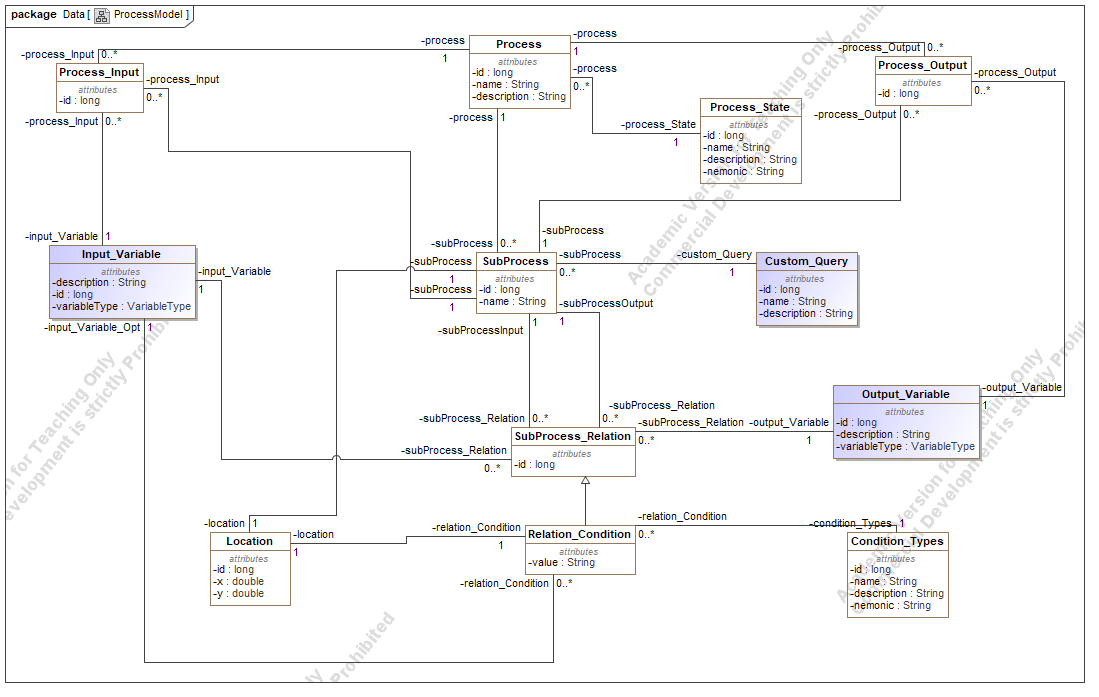
\includegraphics[width=\linewidth]{processModel.png}
	\caption{Modelo de Datos}
	\label{fig:processModel}
\end{figure}

El objetivo de este paso era que LUCA pudiese almacenar los procesos definidos en una base de datos, de manera que éstos fuesen perdurables. Para ello lo primero era definir un modelo conceptual de datos para los procesos. Dicho modelo conceptual se muestra en la Figura~\ref{fig:processModel}. En esta Figura, las clases sombreadas son clases propias del producto LUCA, a las que referencian las clases creadas  en este proyecto.

El modelo consta de una clase principal llamada Process, esta es la encargada de albergar todos los datos necesarios para poder crear un proceso, tiene establecida un estado (para determinar si es un proceso preparado para ser ejecutado o no, o si ha sido eliminado), se compone de una lista de las variables de entrada y de salida, se decriben a raíz del subproceso al que pertenecen y la variable de entrada o de salida que conecta. El proceso contiene a su vez una la lista de subprocesos. Un SubProceso tiene asociada una consulta, que será la que se ejecute una vez definido el process. Cada enlace entre subprocesos y entre el subproceso y el proceso, se persiste gracias a un SubProcessRelation, este simula un enlace, y por lo tanto contiene la información de las variables de los procesos que conecta, además, existe otra variante de él, el RelationCondition, el cuál informa de un enlace hacia un nodo de condición, por lo tanto también alberga la variable del nuevo subproceso al que conecta.
%%==============================================================================%%
%% NOTA(Pablo): Describir un poco el modelo desde texto
%%==============================================================================%%


Este modelo conceptual de datos fue implementado en \emph{Java}, utilizando POJOs (\emph{Plain Old Java Objects}) y posteriormente anotado usando \emph{JPA (Java Persistence API)}~\cite{jpa} para indicar cómo debían crearse las tablas de la base de datos relacional que daría soporte a dicho modelo. De esta forma, es \emph{JPA} quién automáticamente creará el esquema de base de datos, así como las interfaces de los repositorios pertinentes para manipular los objetos de negocio definidos por nuestro modelo conceptual de datos. Además, esta herramienta asegura el correcto funcionamiento de la capa de persistencia, por lo tanto no siendo necesario crear pruebas a este nivel.

Una vez creado este modelo conceptual de datos, la capa de negocio se subdividió en dos subcapas. La primera era la capa de \emph{control de acceso} y se encargaría de verificar que quién desea utilizar la capa de negocio posea los privilegios y permisos necesarios para hacerlo. La segunda subcapa era la propia capa de negocio, que gestiona los procesos y los diferentes elementos que posee el modelo. Para ello esta capa se comunica con una capa de persistencia que utiliza por debajo \emph{JPA} para la comunicación con la base de datos relacional.

%% ejemplo controlador
\begin{figure}[H]
	\centering
	\begin{lstlisting}[language=Java]
	@PreAuthorize(ProcessPermission.AUTH_PROCESS_CREATE)
	Process saveProcess(Process process);\end{lstlisting}
	\caption{Interfaz controladora}
	\label{fig:interfazControladora}
\end{figure}

\begin{figure}[H]
	\centering
	\begin{lstlisting}[language=Java]
	@Autowire
	private ProcessService processService;
	
	@Override
	public Process saveProcess(Process process){
		return processService.saveProcess(process);
	}\end{lstlisting}
	\caption{Implementación interfaz controladora}
	\label{fig:interfazControladoraImpl}
\end{figure}

La Figura~\ref{fig:interfazControladora} muestra cómo se verifican los permisos y privilegios del usuario que utiliza el servicio. Para llevarlo a cabo, se comprueba previo a la ejecución del método, que el usuario tiene en este caso los permisos para crear un proceso. Una vez verificados esos permisos, se ejecuta el método. Internamente, se llama al servicio propio de la capa de negocio para realizar la operación de persistencia (Figura~\ref{fig:interfazControladoraImpl}).

En las consecutivas iteraciones se fueron añadiendo las funcionalidades necesarias para poder persistir el modelo de datos conforme este se iba enriqueciendo en las sucesivas iteraciones. 

\begin{figure}[H]
	\centering
	\begin{lstlisting}[language=Javascript]
	INSERT INTO
	LUCA_PROCESSES(id,DESCRIPTION,NAME...)
	VALUES(2,'process_test_desc','process_test_name',...\end{lstlisting}
	\caption{Fichero \emph{SQL}}
	\label{fig:sqlFile}
\end{figure}

Para la capa de servicio si fue posible definir pruebas automatizadas, ya que se crearon test para todos los métodos asociados a la persistencia del modelo. Para realizarlas se utilizó conjuntamente la capa de repositorio, de forma que fue necesario introducir datos en la base de datos previos a cada test. Esto se realizó mediante un fichero \emph{SQL} (Figura~\ref{fig:sqlFile}) que al inicio de cada test cargaba diversos datos en la base de datos y al final de cada test la vacíaba. De esta forma dicha base de datos queda preparada para la consecutiva ejecución de pruebas sin depender de las anteriores.

\begin{figure}[H]
	\centering
	\begin{lstlisting}[language=Javascript]
	@Test
	@Sql(value = "classpath:ProcessTestsIT.sql")
	public void testGetProcesses()
	{
		PageRequest pageRequest = null;
		ProcessFilter filter = new ProcessFilter();
		List<Process> processes = processService.
		getProcess(filter, pageRequest).asItemsList();
		
		assertTrue(processes.size() == 2);
	}\end{lstlisting}
	\caption{Ejemplo Test}
	\label{fig:testExample}
\end{figure}


La Figura~\ref{fig:testExample} muestra el caso de prueba para la obtención de todos los \emph{Procesos} existentes en la base de datos. En éste se puede comprobar como se importa el fichero \emph{SQL} (Figura~\ref{fig:testExample}, Línea 2), y luego se simula una petición a la base de datos a través del servicio apropiado (Figura~\ref{fig:testExample}, Líneas 5-8). Finalmente se comprueba que se han recibido todos los datos esperados (Figura~\ref{fig:testExample}, Línea 10). En este ejemplo se usa el concepto de filtro, el cuál permite (como su propio nombre indica) filtrar en función de las propiedades de un \emph{proceso}. Por ejemplo, si en el filtro se introduce un identificador, solo se traerá el \emph{proceso} coincidente con dicho identificador.

\begin{figure}[H]
	\centering
	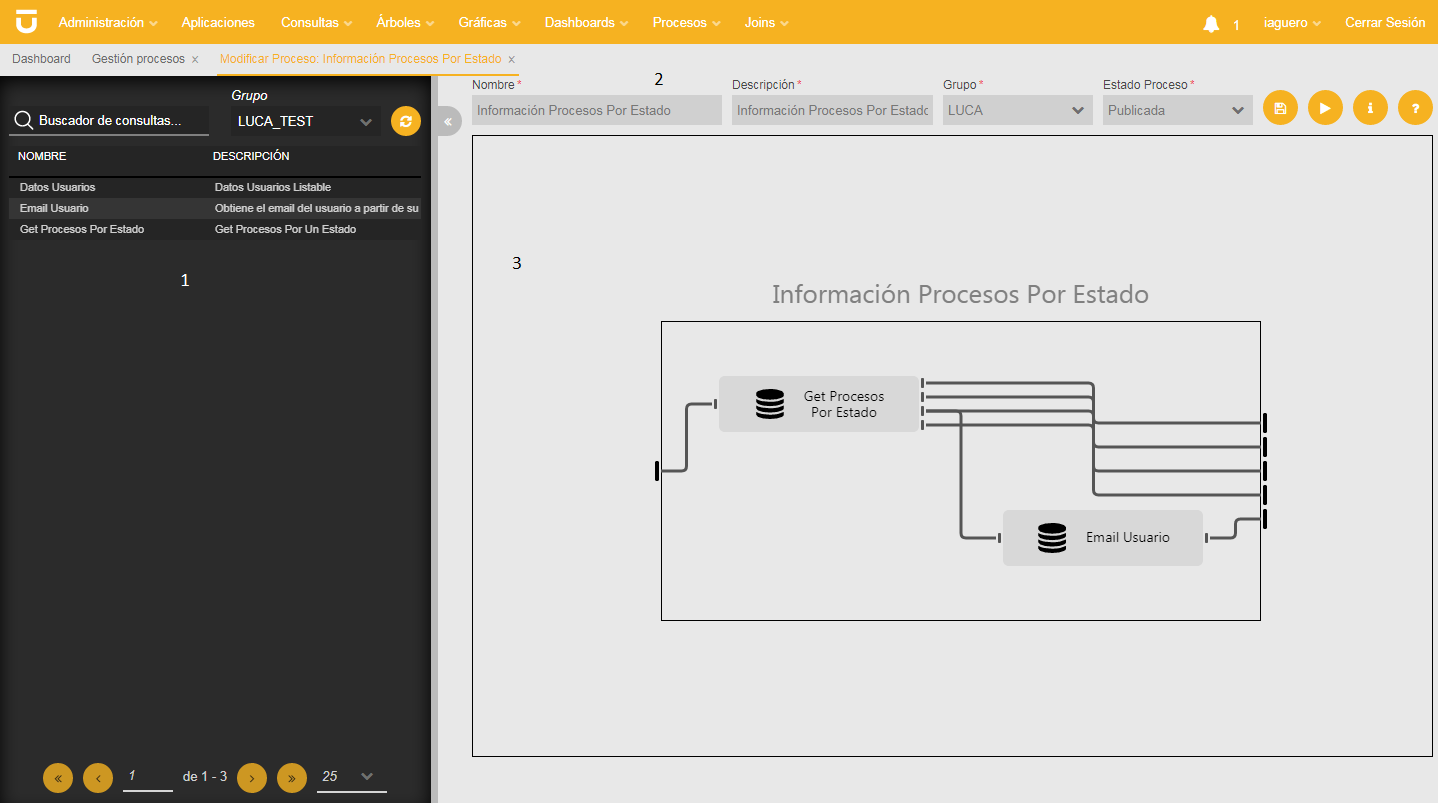
\includegraphics[width=\linewidth]{capturasLuca/gestionProceso.png}
	\caption{Creación de un proceso}
	\label{fig:gestionProceso}
\end{figure}

La Figura~\ref{fig:gestionProceso} ilustra, para cerrar la descripción del editor gráfico, la interfaz de creación de un proceso. La interfaz se compone de tres secciones bien diferenciadas, por una parte tenemos una tabla con las diferentes consultas que pueden ser utilizadas en el proceso. Esta tabla además, puede ser filtrada en base al grupo al que queremos que pertenezcan las consultas (Figura~\ref{fig:gestionProceso}, etiqueta 1). La sección superior de la figura (Figura~\ref{fig:gestionProceso}, etiqueta 2) muestra todas las características necesarias para crear un proceso. La última sección alberga el diagrama con el que el usuario puede interactuar para construir el proceso utilizando las diferentes consultas que son arrastradas desde la tabla de consultas (Figura~\ref{fig:gestionProceso}, etiqueta 3).

\begin{figure}[H]
	\centering
	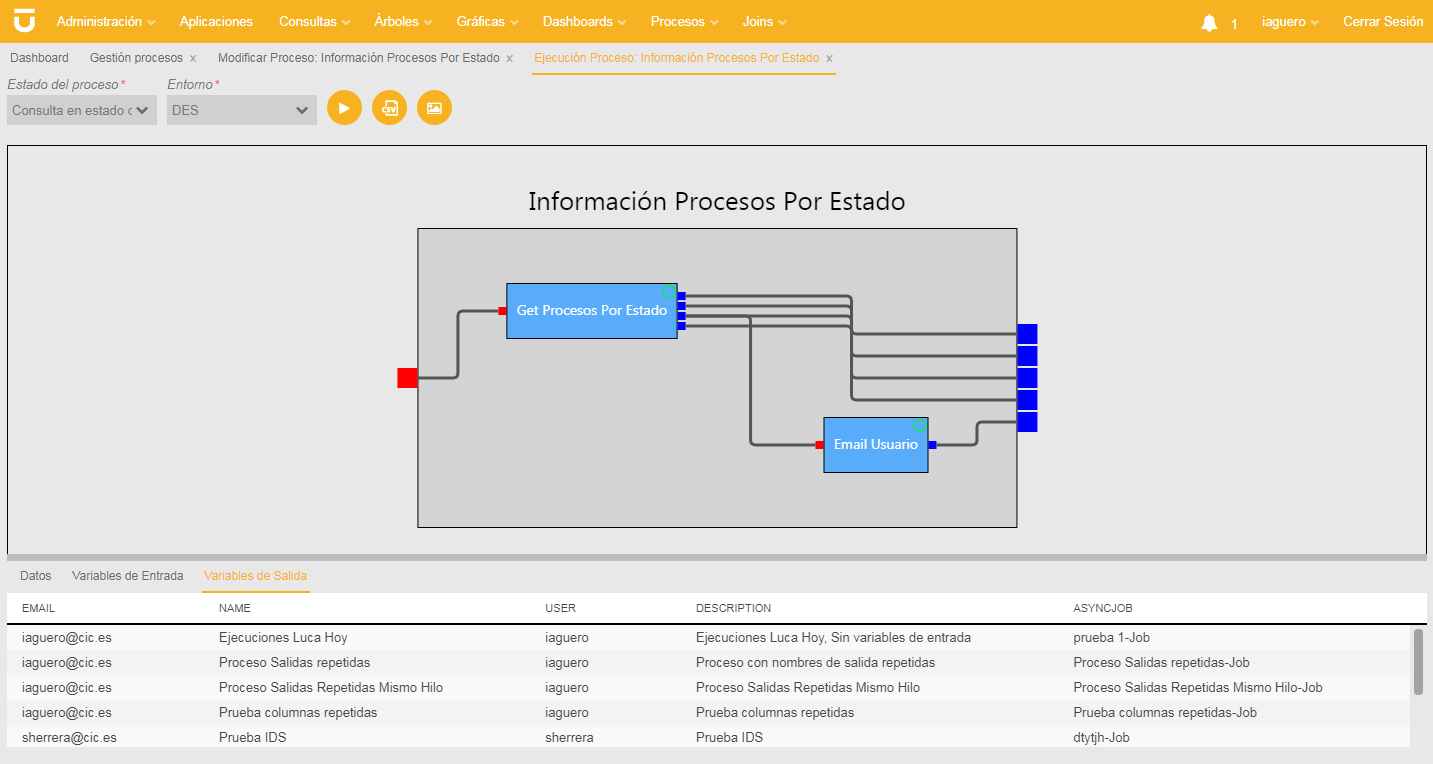
\includegraphics[width=\linewidth]{capturasLuca/ejecucionProceso.png}
	\caption{Ejecución de un proceso}
	\label{fig:ejecucionProceso}
\end{figure}

\section{Ejecución de Procesos}

%%==============================================================================%%
%% NOTA(Pablo): Describir aquí un poco a nivel técnico cómo se ejecuta un 
%%    proceso y poner algo de código relativo a la ejecución de los procesos
%%==============================================================================%%


Para finalizar, la Figura~\ref{fig:ejecucionProceso} muestra la ejecución de un proceso. Esta figura se puede dividir en tres secciones. La primera consta de los campos necesarios para poder ejecutar un proceso (Figura~\ref{fig:ejecucionProceso}, etiqueta 1). En la segunda sección se muestra el diagrama del proceso (esta vez no es editable), en él, durante la ejecución, se podrá ir visualizando el flujo de ejecución del proceso, viendo que consultas o enlaces se han ejecutado correctamente o no (Figura~\ref{fig:ejecucionProceso}, etiqueta 2). La última sección muestra el resultado de ejecutar el proceso, se visualiza una tabla con el conjunto de resultados (Figura~\ref{fig:ejecucionProceso}, etiqueta 3). Además de estas secciones, el usuario si lo desea puede ocultar el diagrama para solo visualizar la tabla de resultados(Figura~\ref{fig:ejecucionProceso}, etiqueta 4).




